%% This is file `elsarticle-template-1-num.tex',
%%
%% Copyright 2009 Elsevier Ltd
%%
%% This file is part of the 'Elsarticle Bundle'.
%% ---------------------------------------------
%%
%% It may be distributed under the conditions of the LaTeX Project Public
%% License, either version 1.2 of this license or (at your option) any
%% later version.  The latest version of this license is in
%%    http://www.latex-project.org/lppl.txt
%% and version 1.2 or later is part of all distributions of LaTeX
%% version 1999/12/01 or later.
%%
%% Template article for Elsevier's document class `elsarticle'
%% with numbered style bibliographic references
%%
%% $Id: elsarticle-template-1-num.tex 149 2009-10-08 05:01:15Z rishi $
%% $URL: http://lenova.river-valley.com/svn/elsbst/trunk/elsarticle-template-1-num.tex $
%%

%% Use the option review to obtain double line spacing
%% \documentclass[preprint,review,12pt]{elsarticle}

%% Use the options 1p,twocolumn; 3p; 3p,twocolumn; 5p; or 5p,twocolumn
%% for a journal layout:
%% \documentclass[final,1p,times]{elsarticle}
%% \documentclass[final,1p,times,twocolumn]{elsarticle}
%% \documentclass[final,3p,times]{elsarticle}
%% \documentclass[final,3p,times,twocolumn]{elsarticle}
%% \documentclass[final,5p,times]{elsarticle}
%% \documentclass[final,5p,times,twocolumn]{elsarticle}

\documentclass[12pt,authoryear]{elsarticle}

\makeatletter
\def\ps@pprintTitle{%
 \let\@oddhead\@empty
 \let\@evenhead\@empty
 \def\@oddfoot{\centerline{\thepage}}%
 \let\@evenfoot\@oddfoot}
\makeatother

%% Language and font encodings
\usepackage[english]{babel}
\usepackage[utf8x]{inputenc}
\usepackage[T1]{fontenc}
\usepackage[document]{ragged2e}
\usepackage{setspace}

%% Sets page size and margins
\usepackage[a4paper,top=3cm,bottom=3cm,left=3cm,right=3cm,marginparwidth=1cm]{geometry}
\usepackage{lscape}

%% Useful packages
\usepackage{amsmath}
\usepackage[colorinlistoftodos]{todonotes}
\usepackage[colorlinks=true, allcolors=blue]{hyperref}
%Prevents that citations cross the margin of the manuscript
\usepackage{breakcites}
\usepackage{float}
\newcommand{\ackname}{Acknowledgements}

%% The lineno packages adds line numbers. Start line numbering with
%% \begin{linenumbers}, end it with \end{linenumbers}. Or switch it on
%% for the whole article with \linenumbers after \end{frontmatter}.
\usepackage{lineno}
%\linenumbers

%% Table packages
\usepackage{a4wide}
\usepackage{enumitem}
\usepackage{array}
\usepackage{rotating}
\usepackage{booktabs}
\usepackage{multirow}% http://ctan.org/pkg/multirow
\usepackage{hhline}% http://ctan.org/pkg/hhline
\usepackage{adjustbox}
\usepackage{graphics}
%% The graphicx package provides the includegraphics command.
\usepackage{graphicx}

%% Figure Packages
\usepackage[font={small,it}]{caption}
\setcounter{secnumdepth}{4}

%% The amssymb package provides various useful mathematical symbols
\usepackage{amssymb}
%% The amsthm package provides extended theorem environments
%% \usepackage{amsthm}

%% natbib.sty is loaded by default. However, natbib options can be
%% provided with \biboptions{...} command. Following options are
%% valid:

%%   round  -  round parentheses are used (default)
%%   square -  square brackets are used   [option]
%%   curly  -  curly braces are used      {option}
%%   angle  -  angle brackets are used    <option>
%%   semicolon  -  multiple citations separated by semi-colon
%%   colon  - same as semicolon, an earlier confusion
%%   comma  -  separated by comma
%%   numbers-  selects numerical citations
%%   super  -  numerical citations as superscripts
%%   sort   -  sorts multiple citations according to order in ref. list
%%   sort&compress   -  like sort, but also compresses numerical citations
%%   compress - compresses without sorting
%%
%% \biboptions{comma,round}

% \biboptions{}

\journal{Science of the Total Environment}

\begin{document}
%double spacing to facilitate the reviewing process
\doublespacing

\begin{frontmatter}

%% Title, authors and addresses

\title{%
Implications of movement for species distribution models \\
\large Rethinking environmental data tools\\
\small February 2018}

%% use the tnoteref command within \title for footnotes;
%% use the tnotetext command for the associated footnote;
%% use the fnref command within \author or \address for footnotes;
%% use the fntext command for the associated footnote;
%% use the corref command within \author for corresponding author footnotes;
%% use the cortext command for the associated footnote;
%% use the ead command for the email address,
%% and the form \ead[url] for the home page:
%%
%% \title{Title\tnoteref{label1}}
%% \tnotetext[label1]{}
%% \author{Name\corref{cor1}\fnref{label2}}
%% \ead{email address}
%% \ead[url]{home page}
%% \fntext[label2]{}
%% \cortext[cor1]{}
%% \address{Address\fnref{label3}}
%% \fntext[label3]{}


%% use optional labels to link authors explicitly to addresses:
%% \author[label1,label2]{<author name>}
%% \address[label1]{<address>}
%% \address[label2]{<address>}

\author{Stijn Bruneel$^{1,2\ast}$, Sacha Gobeyn$^{1}$, Pieterjan Verhelst$^{1,2,3,4}$, Jan Reubens$^{4}$, Tom Moens$^{2}$, Peter Goethals$^{1}$}

\address{$^{1}$Department of Animal Science and Aquatic Ecology, Ghent University, Coupure Links 653, 9000 Ghent, Belgium,

$^{2}$Marine Biology Research Group, Ghent University, Krijgslaan 281, 9000 Ghent, Belgium,

$^{3}$Research Institute for Nature and Forest (INBO), Havenlaan 88, bus 73, 1000 Brussels, Belgium,

$^{4}$Flanders Marine Institute (VLIZ), Wandelaarkaai 7, 8400 Ostend, Belgium

$^\ast$To whom correspondence should be addressed; E-mail: stijn.bruneel@ugent.be}

\begin{abstract}
%% Text of abstract
Movement is considered an essential process in shaping the distributions of species. Nevertheless, most species distribution models (SDMs) still focus solely on environment-species relationships to predict the occurrence of species. Furthermore, the currently used indirect estimates of movement allow to assess habitat accessibility, but do not provide an accurate description of movement. Better proxies of movement are needed to assess the dispersal potential of individual species and to gain a more practical insight in the interconnectivity of communities. Telemetry techniques are rapidly evolving and highly capable to provide explicit descriptions of movement, but their usefulness for SDMs will mainly depend on the ability of these models to deal with hitherto unconsidered ecological processes. More specifically, the integration of movement is likely to affect the environmental data requirements as the connection between environmental and biological data is crucial to provide reliable results. Mobility implies the occupancy of a continuum of space, hence an adequate representation of both geographical and environmental space is paramount to study mobile species distributions. In this context, environmental models, remote sensing techniques and animal-borne environmental sensors are discussed as potential techniques to obtain suitable environmental data. In order to provide an in-depth review of the aforementioned methods, we have chosen to use the modelling of fish distributions as a case study. The high mobility of fish and the often highly variable nature of the aquatic environment generally complicate model development, making it an adequate subject for research. Furthermore, insight into the distribution of fish is of great interest for fish stock assessments and water management worldwide, underlining its practical relevance.
\end{abstract}

\begin{keyword}
species distributions \sep fish movement \sep environmental data collection \sep telemetry
%% keywords here, in the form: keyword \sep keyword

%% MSC codes here, in the form: \MSC code \sep code
%% or \MSC[2008] code \sep code (2000 is the default)

\end{keyword}

\end{frontmatter}

%% main text

%%
%% Start line numbering here 
%%
%\linenumbers

\section{Introduction}
\label{Introduction}

The distribution of species and communities in space has been a major focus of study in ecological research \citep{Austin2002,Guisan2005,Elith2009}. In order to assess how species will be affected by climate change \citep{Ramirez-Villegas2014,Dulvy2008,Austin2011} or how current species distributions came to be \citep{Wiens2004,Varela2011}, a firm understanding of the functional relationships between species and the environment is required. Ecological traits of species, which are associated with the preference for specific environmental conditions, are key to understand why species prefer one habitat over the other \citep{Stoll2014}. In general, these habitat preferences are described as correlative species-environment relationships using habitat suitability models (HSMs) also often referred to as species distribution models (SDMs). However, in a strict sense of the word, the suitability of a habitat for a certain species does not necessarily imply the presence of that species \citep{Meynard2013}. Besides ecological traits, species also own a wide set of biological traits \citep{Costello2015}. Biological traits are referred to as the physiological and behavioral characteristics of a species and include among others the ability to interact and to disperse \citep{Costello2015}. SDMs aim to predict the distribution of species, but to do so they need to account for both the ecological and biological traits of species \citep{Forio2017,Verberk2010}. 

In the context of SDMs, the term dispersal is often used instead of movement, mainly because the accessibility of habitats by species or populations is considered rather than the underlying process of movement itself \citep{Datry2016,Austin2002,Elith2006,Guisan2005}. Dispersal can as such be defined as the cumulative movement of a species or population between habitats over a longer period \citep{Soberon2005,Guisan2005,Holloway2016}. However, there is more to movement than merely being in function of tracking and reaching suitable habitats. First, habitats are seldom well-aligned areas with constant borders in time within which populations remain stationary. The scale at which habitats are observed may allow to approximate habitats as well-aligned points in space rather than complex areas, but this depends on the characteristics of the studied ecosystem. Second, characteristics of the movement of individuals may in fact be necessary to provide a sound description of movement-related biological traits and to distinguish dispersal from other types of movement such as migration or within-habitat-displacement. Movement in SDMs is currently described as a population-based post hoc derivative of movement with binary response (habitats are or are not accessible) \citep{Guisan2006}, but being able to label and quantify movement more directly, may entail more realistic predictions and quantifications of uncertainty \citep{Holloway2016,Uribe-Rivera2017,Singer2016,Dedecker2006}. 

The level-up of biotic data quality, driven by technological advancements in biotic data acquisition techniques, is expected to stimulate the integration of movement in SDMs \citep{Guisan2005,Thuiller2013}. Such models are potentially much more powerful in explaining observed species distributions than the more traditional SDMs which only incorporate environment-species relationships. An important issue that should be kept in mind in this evolution of models is how the currently used abiotic data acquisition techniques impact the overall quality of the model outcomes. In other words: How is model accuracy influenced by the quality of environmental data? Before addressing this issue, we first require some insight into the development of SDMs and the new sampling technologies. After having identified the deficiencies of current SDMs and the potential of new technologies to deal with them, we discuss new challenges and propose some ways to tackle them. 

\vspace{5mm}

The importance of upscaling biological data quality with more detailed movement data depends on the studied species and ecosystem \citep{Thuiller2015}. For sessile organisms, like most macroinvertebrates, the issue of integrating distance-related biological processes may be less pressing than for more mobile species. Fish are typically mobile species and thus their movement may be of great importance for their geographical distributions. Furthermore, as some aquatic habitats are spatially and temporally very dynamic, the quality of environmental data is also expected to play an essential role in the accuracy of SDMs. A central assumption in traditional SDMs is that species are in equilibrium with their environment \citep{Araujo2005,Elith2010}. However, this might not necessarily be the case in dynamic environments such as tropical forests, estuaries and anthropogenically influenced areas. After fire disturbances for example, species are unlikely to be in equilibrium with the disturbed environment \citep{Tucker2012}. The scale of the disturbance in relation to the spatial structure of plant populations, associated with seed dispersal and seed bank characteristics, will determine if a species will be able to persist, reestablish itself or be excluded from the habitat. Another key example involves climate change which might drive populations to extinction due to rapidly changing environmental conditions and lacking interconnectivity between suitable patches \citep{Araujo2005,Travis2013,Sinclair2010}. Furthermore, insights into the movement pathways, movement limitations, ecological and biological traits of invasive species are vital to predict their future distributions and to adapt biodiversity policies accordingly \citep{Gallien2012,Boets2014}. Hence, it is expected that the quality of SDMs for mobile species in dynamic environments will strongly depend on the integration of movement and the quality of used environmental data. 

In order to provide a sufficiently in-depth example of evolving sampling techniques, we have chosen to limit the sections on biotic and abiotic data acquisition and processing to fish distribution research. This field of research is witnessing some rapid advancements in biotic sampling techniques, providing an interesting case study and insight in how these evolutions alter conceptual modelling frameworks and data requirements \citep{Hussey2015,Donaldson2014,Metcalfe2012}. Nevertheless, most of the discussed conceptual approaches, techniques and repercussions for model developers can still be viewed in a broader sense, comprising not only the biosphere and hydrosphere but all environmental matrices sustaining life.

\section{Model Conceptualization}
\label{Model:Conceptualization}

The procedure of building ecological models consists of conceptualization, data acquisition and preprocessing, model fitting, model evaluation, spatial predictions and assessment of model applicability \citep{Guisan2000}. An essential starting point for every model is the delineation of the underlying ecological concept and its derivatives to serve as a framework \citep{Guisan2000}.

The distribution of a species is the result of a set of abiotic and biotic hierarchical filters which act upon the traits of the concerned species \citep{Austin2002}. Environmental conditions and biotic interactions will act as a series of filters, determining if species will be present or absent. Environmental conditions, steered by for instance temperature and dissolved oxygen (DO) concentration, are selective on the physiological tolerance of species. Biotic interactions on the other hand will act upon the ability of species to endure and profit from competition and predation, introducing another selective force on the occurrence of a species. Hutchinson (1957) made a distinction between the effects of these two types of filters by introducing the terms fundamental and realized niches\nocite{Hutchinson1957}. The fundamental niche is delineated by environmental constraints, while realized niches additionally include biotic interactions, usually resulting in a considerably smaller niche than when only environmental filters are considered \citep{Guisan2000}. In this filter/niche theory, movement is not explicitly included, although many studies have found that over ecologically relatively large scales movement, rather than biotic interaction, is determinative for species distributions \citep{Guisan2005,Soberon2005,Peters2005,Peterson2006}. 

Especially in metacommunity ecology, dispersal-related movement is considered a prime driver of interconnection between local communities. Dispersal allows species to track and respond to differences in environmental conditions and assemblages of interacting species across landscapes \citep{Leibold2004}. The dispersal potential of a species is a trait that might either weaken or strengthen the effects of biotic interaction and environmental conditions \citep{Leibold2017}. For example, species with a strong ability to colonize or to compete for resources, might not meet the full potential of their ability due to low dispersal rates or dispersal limitations \citep{Heino2015}. In other cases however, mass effects may take place when dispersal rates become so high that species settle in unsuitable habitats \citep{Heino2015}. The species might not thrive in this sink habitat, but might be prevented from extinction due to dispersal from the source habitat \citep{Heino2015}.

Movement of a species is not only associated with its dispersal rate or the physical accessibility to any suitable habitat, but it is also closely linked to the environmental conditions and biotic interactions. Changing environmental conditions, encounters with predators and migrations of prey might all drive the movement of a species. Although both biotic interactions and movement are intertwined and can be considered as distance-related biological processes, the relatively large scale, importance of orientation in geographical space and time-dependent nature of movement, have caused it to be defined as a spatial factor rather than a niche factor \citep{Araujo2006,Guisan2006}. In order to evaluate the conceptual requirements of any model incorporating movement, the different aspects which differentiate movement as a spatial factor from the different niche factors should be discussed first. In figure \ref{fig:Figure1}, this conceptual difference of spatial and niche factors is depicted. Most researchers nowadays have acknowledged the importance of both niche and spatial factors, but only few have tried to combine them in ecological models \citep{Franklin2010,Peterson2011}. 

\begin{figure}[!ht]
  \centering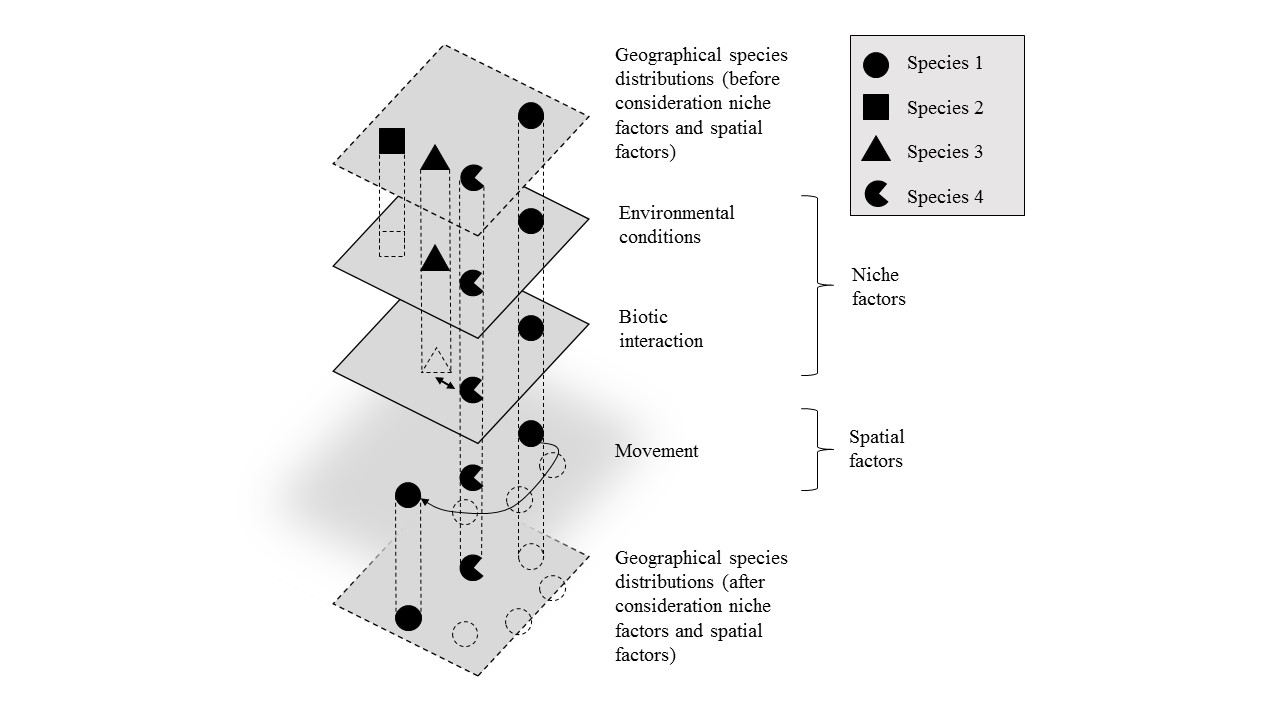
\includegraphics[scale=0.45]{Figure1}
  \caption{Distinction between niche factors (environmental conditions and biotic interactions) and spatial factors (movement). The layers visualize the geographical species distributions after considering environmental conditions, biotic interaction and movement respectively. The different species are depicted as different geometric figures. In this figure the way in which niche factors and spatial factors influence species distributions, is represented in a simplified manner. For example, environmental conditions allow for species 1, 3 and 4 to endure while species 2 is not able to persist in the considered environment. Species 2 is not adapted as well to the current environmental conditions as species 1, 3 and 4. When taking into account species interactions , species 1 and 4 endure while species 3 does not. This is due to predation of species 3 by species 4. The geographical species distributions, realized after consideration of the niche factors, can be visualized as well-aligned geographical layers where the species distributions are represented as present/absent points with fixed spatial orientations. This is visualized by the full border line of the two layers. However, when considering movement, species can by definition not be represented as objects with a fixed spatial orientation. The unclear borders of geographical space represent the geographical reality, in which the spatial orientation of a species over time is in fact a continuum rather than a fixed location. This difference between niche factors and spatial factors is key to understand the required adaptations in future conceptual frameworks of models dealing with movement.}
  \label{fig:Figure1}
\end{figure}

\vspace{5mm}

In the past, when the effects of movement were neglected, there was no incentive to integrate geographical influences in SDMs and only environmental space was considered to predict geographical distributions of species. Environmental space can be considered as a n-dimensional space, with each variable being represented by one dimension. Geographical space on the other hand consists of no more than three dimensions representing the physical space in which movement occurs. The artificial nature of solely focusing on environmental space becomes clear when breaking down the different basic modelling steps. Species are stripped from their orientation in geographical space, linked to a subset of environmental variables, and then refitted through species-environment relationships in geographical space. As such, an estimation of geographical species distributions is obtained. 

Inherent to the definition of space is the description of scale. Scale can be divided into the grain size (or resolution), representing the unit of analysis, and the extent, which defines the scope of the analysis \citep{Song2013}. Many researchers have already stressed the importance of a good relational basis in time and space between species and environmental layers \citep{Fernandez2013,Elith2009}, but only few of these concerns have been acknowledged let alone integrated in SDMs. The earliest referrals to the niche concept as a n-dimensional environmental space not only ignored geographical space but also the importance of spatial and temporal scale \citep{Austin2002}. Even nowadays, the choice for a certain resolution is motivated more by data availability rather than the environmental and biological processes and their associated range of influence \citep{Guisan2005,Yackulic2016,Song2013}. The hierarchy of the influencing environmental variables, which drives the patterns of species distributions, will vary according to changes in scale \citep{Pearson2004,Guisan2005}. Therefore, extrapolating relationships without consideration of the used scale will likely result in ambiguous findings. The importance of scale becomes even more clear when movement and biotic interaction are considered. These processes are thought to be important on different scales, ranging from a fine scale for biotic interactions, to an intermediate scale for movement and a large scale for environmental filters \citep{Thuiller2015,Guisan2005}. 

Acknowledging that geographical space and scale are imperative to the future advancements of SDMs is a first step towards an adequate integration of movement in SDMs. As the conceptualization therefore requires changes, so will the consecutive steps of the SDM development process need to adapt.

\section{Data acquisition and preprocessing}

As we move away from a conceptual model that focuses on species distributions affected by environmental conditions alone, we should evaluate how the requirements for the environmental data will be affected by such a change. In other words, we want to know how recent advancements in biotic sampling technology and improvements of biotic data quality and format might influence the requirements for abiotic data. Therefore, the focus should first be set on biotic sampling techniques, the data they provide and how they can be processed. It makes sense that the characteristics of considered biotic processes will at least partially dictate the format of the required environmental data. Finally, the assessment, evaluation and perhaps rethinking of the currently used techniques for environmental data acquisition and processing will be discussed.

\subsection{Biotic data: Focusing on fish as mobile species}

\subsubsection{Biotic data collection}
\label{Biotic:data:collection}

To optimally exploit the information stored in the biological data sets, the choice of abiotic data acquisition and processing tools should be guided by the characteristics of the biological data. The conceptual shift in the biological data from a population to an individual based approach has an intellectual motivation as movement has been recognized as an important process in SDM development \citep{Soberon2005,Holloway2016}. It is, however, the relatively recent evolution in biological data acquisition techniques that has led to enhanced spatial and temporal resolutions and has allowed a better understanding of the behaviour (movement and biotic interactions) of single individuals \citep{Hussey2015}.

Traditional biotic data acquisition methods which involve manual capturing such as fyke, trawl and electrofishing sampling, are characterized by a rather limited spatial and temporal coverage of the area of interest. Fykes generally have a low sampling efficiency, are size-selective, are influenced by fish already trapped and only provide a cumulative measure of the amount of fish present. These aspects make the accuracy of any prediction on the occurrence of a species strongly dependent on temporal variability and sampling time intervals \citep{Clavero2006}. Trawl samples on the other hand, being active methods to collect fish in a relatively short time compared to fykes, are less sensitive to temporal variation. However, the loss of independence between locations along the tow transect requires some correction for pseudo-replication and spatial autocorrelation \citep{Dormann2007,Elith2009}. Another often applied method is electrofishing, which, however, depends strongly on water salinity, depth and whether the fish have swim bladders or not \citep{Clavero2006,Reyjol2005}. Therefore, to avoid biases, corrections should be made to account for different environmental conditions and different tolerances against electrical currents of different fish species. 

Techniques which are less disruptive and extractive than fykes, trawls and electrofishing are gaining importance. A first example, involves the use of environmental DNA (eDNA). eDNA is defined as genetic material obtained directly from environmental samples \citep{Thomsen2015}. It has been used in both freshwater and marine ecosystems to detect aquatic species and recent studies suggest the method can also be used to estimate relative abundances \citep{Lacoursiere-Roussel2016,Baldigo2017,Thomsen2012}. Although, the amount of field-based studies is still limited \citep{Sassoubre2016} and the behaviour of eDNA in the water column has only been given few consideration \citep{Shogren2017,Dejean2011}, it is a promising method to efficiently obtain insights in species assemblages \citep{Thomsen2015}. The method may be especially useful to assess the presence of rare species, which are difficult to determine through traditional extractive methods \citep{Laramie2015,Weltz2017,Wilcox2013,Pfleger2016}. A second approach allowing non-destructive assessments of fish assemblages involves underwater visual census (UVC) and video monitoring. UVC has been used in marine areas for over sixty years, but is becoming overshadowed by the rapidly evolving video monitoring techniques \citep{Mallet2014}. Their potential for high replication and non-obtrusive nature have stimulated the development of a wide collection of set-ups in different areas \citep{Mallet2014,Neuswanger2016}. Although low visibility in certain areas may hamper the applicability of video techniques, different video-setups, ranging from diver operated to towed video systems and (baited) remote video stations, have proven useful in coral reefs, tropical rivers and even dynamic estuaries \citep{Mallet2014,Schmid2017,Wartenberg2015,Zintzen2012}. 

\vspace{5mm}

The aforementioned methods may provide interesting insights into species distributions, but their inability to translate the collected biological data to the level of individuals and to explicitly account for their movement is a major limitation. Implementing a direct quantification of dispersal and dispersal ability, could significantly improve the practical use of metacommunity concepts \citep{Heino2015,Jacobson2010}. Genetic techniques are commonly used to study longterm dispersal patterns by assessing genetic differences and gene flows among populations \citep{Hughes2007}. However, these post hoc methods require sufficient basic knowledge on the natural history of aquatic species, communities and their environment to disentangle the influence of biotic interactions, environmental filtering and dispersal on current species assemblages \citep{Jacobson2010}. Therefore, they do not necessarily provide a direct estimate of dispersal. The individual-based approach of telemetry could provide a much clearer insight into the dispersal ability of tagged species \citep{Thorstad2013}. However, there are some implications involved. First, telemetry studies are typically limited to a subset of species, while metacommunities generally consist of dozens of species \citep{Heino2015}. Second, telemetry does not provide an estimate of the size of a population, but focuses on only a few individuals instead. Hence, a combination of aforementioned techniques would still be required to provide the necessary insights into species distributions by targeting different aspects of the studied communities \citep{Emmrich2010}. 

\vspace{5mm}

Telemetry can broadly be defined as all methods using either sound, visualizations or electronic tags to obtain information on moving animals \citep{Thorstad2013}. However the term most commonly refers to the use of electronic tags. Different types of electronic tags exist, including radio and acoustic transmitters, archival tags and passive integrated transponder tags (PIT-tags). Depending on the research target, study area and type of tagged organism, some methods may be more suitable than others due to differences and trade-offs in data acquisition, detection range, tagging method, sensitivity to environmental conditions, size, life time, etc. \citep{Thorstad2013}.

Radio telemetry and acoustic telemetry are both active methods, meaning that transmitters independently emit signals at certain time intervals to listening stations \citep{Hussey2015,Donaldson2014}. PIT tags on the other hand are called passive because they have no battery. More specifically, a nearby station powers the tag through radio-frequency (RF) induction after which the unique code of the tag is sent in return \citep{Thorstad2013}. The detections obtained by all three techniques provide direct insight into the movement of the studied animal. 

However, besides emitting signals to track presence, transmitters can also be linked to sensors that measure  environmental variables such as water temperature and salinity or individual characteristics such as heartbeat and swim speed \citep{Thorstad2013}. Archival tags do not emit any signal and therefore should be recaptured or retrieved to acquire the stored data. As data are collected afterwards, no direct real-time locations have been established and researchers need to reconstruct trajectories based on sensor data of water depth, light, temperature, the magnitude of the earth magnetic field stored in the tags, etc. \citep{Thorstad2013,Whoriskey2016,Aarestrup2009}. 

The high diversity in electronic tags, in combination with the rapid advancements in technology and data processing, will likely result in an increasing use of telemetry in fish movement studies. Furthermore, because telemetry has significantly increased the size of the biotic data compared to that of the currently used abiotic data, abiotic data might prove the limiting factor in modelling efforts \citep{Hussey2015}. Hence, in order to assess how aquatic animals interact with their environment, the format, size and quality of the abiotic data should be evaluated against the evolutions in biotic data. 

\subsubsection{Biotic data format}

An important aspect of any sampling technique is the kind of data it provides. Researchers should evaluate how their type of data can yield a representable measure of biological response and how its characteristics coincide with the target of their study. The traditional fish sampling techniques like fykes provide abundance and presence/absence data at fixed locations. From these locations species-environment relationships can be inferred, that can be extrapolated to other locations based on their environmental conditions. This type of biotic data provides insights into populations at certain locations. The presence-only data of telemetry methods, on the other hand, allow to reconstruct a comprehensive view on habitat use of a single individual. For each individual, all presences can be connected to yield a single trajectory. The set of trajectories is then aggregated to yield a more population oriented summary \citep{Hefley2016,Pearce2006}. The type of acquired data is therefore very different for traditional methods and telemetry. Telemetry data provide area-based information on a series of single individuals, while data from fykes and trawls render point-based information on a population level.

In theory, presence-absence data are best tailored to assess the suitability of a habitat for a certain species, especially when considering relatively stationary species \citep{Elith2009}. That is why many studies focus on methods to deal with the lack of information on absences in presence-only data through the introduction of pseudo-absences \citep{Pearce2006,Aarts2012,Barbet-Massin2012}. Although absence data may support more robust predictions, more detailed descriptions of fixed study locations and better quantifications of prevalence to put the different sampled locations in perspective, some implications on how absence is described and incorporated remain troublesome \citep{Elith2009}. 

\vspace{5mm}

These implications are mainly associated with the movement of species, which is why they have gradually gained attention as researchers became more convinced of the importance of movement in SDM development. Some researchers have tried to extend the original models, which focus on more or less stationary species, to include more mobile species through the integration of focal and temporal predictors. Focal predictors provide a summary of the nearby environment of a studied location \citep{Bucklin2015}. However, the ambiguity surrounding the concept of absence remains. When a species is not recorded at a certain location, other effects such as inaccessibility may be the real underlying cause of absence (i.e. contingent absence \citep{Jimenez-valverde2008}). Hence, assuming that absence is the exclusive result of habitat unsuitability (environmental absence) may simply be wrong \citep{Miller2010}. Furthermore, the concept of absence relies on the assumption of a dynamic equilibrium in space occupancy which neglects the often time-dependent behaviour of the species and external disturbances both on- and off-site \citep{Elith2009}. This major problem of detectability may be partially resolved through the use of telemetry, which enables the tracking of an individual through time and space. Indeed, telemetry not only provides presence-only data as a simple collection of individual presences in a sea of absences, but it also enables a linkage between every presence/detection in both time and space for each individual. Although the lack of real absence data may hamper habitat suitability description in a strict sense, telemetry studies have the potential to reveal unique insights in how species use their overall environment. 

\vspace{5mm}

Individual Based Models (IBMs), which attempt to describe individual movement in time and space, are used to provide these insights into the behaviour of species using telemetry data \citep{Bauer2013}. Most SDMs generally determine empirical relationships between species distributions and local environmental variables at a relatively fine scale \citep{Hayes2009}. IBMs allow to study species distributions by accounting for environmental and biotic processes operating at a much wider scale, such as storm events and movement. Furthermore, as the associated geographical location of each recording is inherently essential to the spatially-explicit model, the linkage between geographical and environmental space will also be imperative for qualitative predictions. The need for implementation of wide-scale and geographical oriented behavioral rules, has been a steering force in the development of a wide set of spatially-explicit IBMs \citep{Railsback2013,Grimm2005}, ranging from larval displacement \citep{Daewel2008} to the migration of fish species \citep{Baetens2013,Papastamatiou2013,Pauwels2014} and the foraging behaviour of whales \citep{Dillon2014}. 

Despite the inherently different approaches of the mainly data-driven SDMs and hypothesis-driven IBMs, their conceptual ecological framework and environmental data requirements are still comparable. Both model types intend to describe species distributions using the same ecological processes and therefore have similar data requirements. 

\subsection{Abiotic data collection }

Different techniques exist to collect environmental data. In this section, commonly used environmental data acquisition methods, are compared with a set of potential alternatives (figure~\ref{fig:Figure2}). To get some insight in the abiotic and biotic techniques most commonly used in SDM studies, a subset of publications was analyzed. The focus was limited to SDM studies on fish which integrated movement in some way. The results are visualized in figure \ref{fig:Figure3}. It should be noted that the nature of the studied ecosystem, study objective and species of interest are paramount to identify the most suitable technique. Ecological researchers should be aware of the range of alternative environmental data acquisition techniques and should take time to evaluate the suitability of a certain technique for their research. Therefore, in table \ref{tab:swot} the key aspects of the discussed abiotic methods are summarized.

\begin{figure}[!ht]
  \centering
	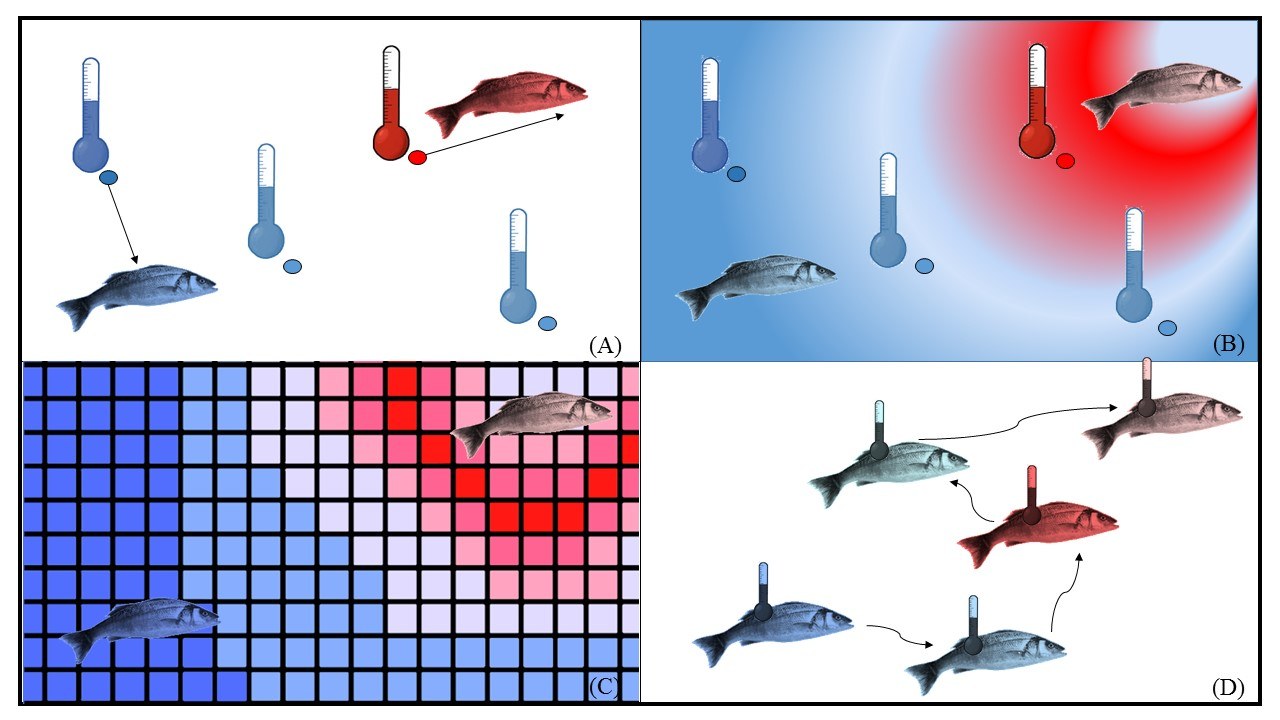
\includegraphics[scale=0.45]{Figure2}
  \caption{Conceptual differences of environmental data acquisition methods. In this figure, temperature is used as example because of its key role as environmental driver of fish distributions worldwide. The thermometers represent temperature and the color gradient from blue to red visualizes the gradient from cold to warm. (A) The locations of the environmental point measurements are chosen independent to the locations at which the fish resides. To represent each fish sampling location the closest environmental point location is chosen. (B) These independent point locations can be combined to produce environmental layers using either interpolation or process-based models. (C) Remote sensing imagery provides environmental layers. The pixel size is associated with the resolution of the remote sensing platform. (D) Animal-borne environmental sensors provide environmental data closely associated to the location of the animal itself. They are therefore referred to as dependent point measurements. For the color version of this figure, we refer the reader to the online version of this paper.}
  \label{fig:Figure2}
\end{figure}

\subsubsection{Independent point-based abiotic data collection and preprocessing}
\label{Indep:Point}

\paragraph{Independent point-based abiotic data collection}\mbox{}\\

Environmental conditions can be measured continuously at fixed locations by the sensors of automated stations or during certain periods of manual field work, using either in-situ or ex-situ methods such as multi-probes or lab analysis, respectively. 

A modern example of an automated mobile measurement station is the Argo float. This device provides temperature and salinity depth profiles at different point locations within a certain grid. By automatically regulating its buoyancy, the float is able to undertake multiple depth cycles. Each time a float surfaces, its data are transmitted to satellites after which it can start a new depth cycle. Another interesting data collection technique is the use of AUV (Autonomous Underwater Vehicles). These devices are able to cover large distances, carry any kind of environmental sensor and navigate with high precision. 

Although Argo floats and AUV are relatively new sampling devices, they share a common independent point-based approach with manual field work and lab analysis. In this review, they are called independent because of their geographical disconnect from biological data collection systems, and point-based because the data they provide originate from point locations. 

\vspace{5mm}

Independent local point-based measurements are the most straightforward and common type of abiotic data collection for SDM development, as the measurements can be coupled directly to biotic sampling locations. For fykes, electrofishing and to a lesser extent trawls, this might seem a justified approach as these methods do not intend to account for movement. The traditional fish sampling techniques yield fish abundances and/or presences/absences at point locations without making assumptions on the areas between the sample locations. Therefore, a point-based coupling between biotic and abiotic data might be an obvious choice. 

However, issues arise for SDM development when considering the mobility of fish and the variability of the environment. In section \ref{Biotic:data:collection} we discussed the inability of traditional fish sampling techniques to monitor movement and proposed telemetry as a complementary technique which does allow to assess fish movement. This technique inherently assumes that tagged organisms use the space between sampling locations, which hampers the applicability of a point-based approach to link environmental conditions to species distributions. Furthermore, randomly selected point measurements alone are often unable to account for geographical dependent variabilities of environmental variables which are generally difficult to identify in aquatic environments due to flow and currents. In addition, many fish SDMs incorporate point measurements of environmental variables taken at locations different from the fish sampling location, to approximate the conditions of each of these fish sampling locations. Although distance is often used as a criterion to allocate abiotic to biotic point locations, such an approach still ignores the importance of orientation in geographical space. Furthermore, it might also inadequately integrate environmental space, depending on the nature of the assessed variable. Despite some efforts to deal with this issue by simultaneously collecting abiotic and biotic data \citep{Maes2007} or by choosing fish sampling locations near abiotic measurement stations, abiotic and biotic point locations often remain insufficiently matched in both time and space \citep{Bultel2014,Currey2015,Stein2015}. 

To deal with the problems of point-based coupling, some preprocessing of data can be done, allowing the format of the abiotic data to coincide with that of the biological processes of interest. This format can generally be pictured as a set of environmental layers able to comply with the concepts discussed in section \ref{Model:Conceptualization}, incorporating geographical space and acknowledging the importance of scale.

\paragraph{Preprocessing of independent point measurements}\mbox{}\\

The independent local point measurements can be transformed into sets of environmental layers. These measurements can be used directly without any prior knowledge, through interpolation or they can be used in combination with acquired hydrodynamical and biogeochemical insights through process-based modelling. Both approaches, although genuinely different, share a common approach in that they both "model" environmental conditions. The environmental conditions measured at certain locations are used to estimate the environmental conditions at other unsampled locations. This implies that these environmental layers are characterized by some degree of model uncertainty, which should be acknowledged during SDM development \citep{Fernandez2013}. Both methods have different sources of uncertainty. Data quality is the most important source of uncertainty in interpolation as it is a data-driven model. Process-based models on the other hand will have a higher degree of uncertainty associated with the model structure. Depending on the nature of each variable, studied ecosystem and target species, either a more data-driven or process-based approach might be preferred. However, because of their complementary nature, a well-considered balance between both approaches is advisable.

\vspace{5mm}

A wide range of interpolation methods have been used with varying success in aquatic environments. Methods include inverse distance weighting (IDW), moving averages, Lagrangian polynomials, loess smoothers, spline, trend and kriging interpolators. The last method has often proven the most useful due to its unique characteristics which render it appropriate for modelling aquatic abiotic variables \citep{Murphy2012,Rathbun1998}. Kriging is generally known as geostatistical interpolation, because of its stochastic nature and its main assumption of spatial correlation between sample points \citep{Calder2009}. 

These two characteristics, stochasticity and spatial correlation, are at the base of the success of kriging. First, unknown values are approximated as a probability distribution rather than a unique value because exact values cannot be determined. Second, this approach, which acknowledges that the unique values can be estimated but not determined, enables the quantification of the estimation uncertainty. Finally, another factor contributing to the wide application of kriging is its stability against violations of assumptions of normality \citep{Rathbun1998}.  

In ordinary kriging, all variability is assumed to originate from the random error term, and no covariates are included. However, when accurate and more or less temporally invariant continuous variables such as latitude, longitude or even bathymetry are available, they are often included to reduce the interval of possible values due to their claim on some of the variability \citep{Urquhart2013,Verfaillie2006,Chehata2007}. This type of interpolation is known as universal kriging and has been found to outperform ordinary kriging, especially in hydrodynamically complex areas \citep{Urquhart2013}. It has also been used extensively to predict DO concentrations in areas with only sparse sampling, using measurements of auxiliary variables such as temperature, salinity and nutrient load \citep{Murphy2013,Zhou2013,Obenour2012,Barabas2001}. We refer readers with a specific interest in these interpolation methods to \citet{Calder2009} and \citet{Webster2008}.

\vspace{5mm}

Process-based models intend to integrate explicit descriptions of dominant processes. The most straightforward processes to model are those of a mainly physical nature, like the hydrodynamics. Hydrodynamic models are mainly described through physical laws, more specifically the mass and continuum conservation laws, which are universally applicable and can be written as partial differential equations \citep{Villars2001}. To solve these complex partial differential equations efficiently, generally numerical models are used. 

Biogeochemical models are less straightforward to integrate, because of the many interacting factors which need to be accounted for. For example, the list of variables which control DO concentration in aquatic systems is extensive and generally includes solar radiance, temperature, salinity, particulate organic matter, reaeration, wind velocity, phytoplankton and zooplankton \citep{Mandal2012}. Hence including every term would lead to a very complex model. Due to this high process complexity, most mechanistic models concerning DO concentration are actually semi-empirical models as they do not integrate all the known underlying processes \citep{Streeter1925}.

\vspace{5 mm}

Both methods, geostatistical interpolation and process-based modelling, have different attractive aspects regarding the integration of movement in SDMs. Geostatistical interpolation is a straightforward technique to produce environmental layers for a wide set of variables which may be very complex to model bottom-up. On the other hand, these basic processes may influence or even determine the movement of species. Integrating these processes explicitly in SDMs might therefore contribute to the identification of important influencing environmental features. 

Nevertheless, some practical limitations remain troublesome. Insufficient and poorly distributed measurement locations in dynamic environments could introduce a significant mismatch of scale between the environmental models and species distribution responses \citep{Fernandez2013}. Furthermore, areas with high ecological relevance such as pools in streams are typically underestimated as the responsible fine-scale processes are often left out due to the risk of overfitting models \citep{Harrison2007}. The spatial and temporal patterns of uncertainty in environmental layers have been acknowledged but only few studies have taken them in consideration \citep{Beale2012,Fernandez2013,Hayes2009}. Although accounting for the introduced uncertainty is crucial, it will not necessarily reduce its direct impact on predictions. Therefore, we should also have a closer look into other methods with a different approach in order to overcome some of the major problems of modelling the environment from independent point-based data. In the following sections, remote sensing and animal-borne sensors will be discussed as promising alternatives for environmental data collection.

\subsubsection{Area-based abiotic data collection}
\label{RS}

Remote sensing can be defined as the science of obtaining information about objects or areas from a distance. This information is acquired in the form of environmental layers and includes images from airborne platforms such as satellites or drones, sonar measurements of bathymetry using boats, etc. In a strict sense this definition also encompasses telemetric tracking of fish, since vocalizations, visualizations and signals emitted through electronic tags are a way of collecting data from a distance. However, to avoid misconceptions in this paper, the term remote sensing will be used for the data acquisition of environmental variables only.

Remote sensing technology has evolved significantly during the last decades and has provided a wide range of environmental sensors and algorithms to process data \citep{He2015}. This evolution has contributed to an increased use of remote sensing data in current species distribution modelling \citep{He2015,Beger2008}. For example, \citet{Goetz2010} used forest heterogeneity, determined with LIDAR remote sensing, to establish a relationship with the occurrence of a bird species. \citet{Gomez2017}  used temperature and chlorophyll a data obtained from the MODIS aqua satellite to delineate priority areas for different whale species. Also \citet{Druon2015} used aqua-MODIS chlorophyll a data to combine with biological traits of European hake to highlight favorable nursery habitats. 

\vspace{5mm}

The major advantage of remote sensing techniques is their ability to produce spatially explicit environmental layers. Interpolation or process-based models use point measurements to infer area-based estimations of environmental conditions, while remote sensing directly provides a synoptic and area-based view of the environment. This area-based view implies a strong link between the acquired environmental data and geographical space, which has been identified as an important feature for the integration of movement in species distribution modelling. Furthermore, the ability to use a spatial multiscale approach while covering an entire area at one single point in time, allows to evaluate the effect of spatial resolution on environmental process description and its relation to species distributions \citep{Pittman2011,Cord2013}. For example, when micro-climate is a determining factor for the occurrence of a certain species, coarse resolution climate data will fail to include essential fine-scale variabilities. On the other hand, when species depend on the overall characteristics of a vast habitat or area, a coarse resolution might be more appropriate in order to distinguish genuine drivers. Consideration of scale and representation in geographical space, which were identified as vital for an optimal assessment of movement, are characteristic for remote sensing techniques \citep{Baban1997}. 

Next to the conceptual requirements when considering movement, the format of biological data should also be evaluated against the characteristics of the environmental data. An important aspect is the delineation between contingent and environmental absences, which in itself is closely associated with the movement of individuals. Remote sensing has the potential to make the distinction between absences caused by environmental conditions and absences caused by movement barriers and local disturbances \citep{Cord2013}. Contingent absences might be distinguished from environmental absences by distinctive features such as differences in bathymetry. Therefore, a strong link with geographical space and an area-based approach are required. Because large areas on a wall-to-wall basis can be covered in relatively small time intervals, it may also be easier to identify, for example, hurdles for movement which might be located further down- or upstream. 

\vspace{5mm}

The major disadvantage of remote sensing techniques is their relatively low temporal resolution due to the time required for full satellite orbits, aircraft availability and cloud cover \citep{Hestir2015,He2015}. As movement is a rather unpredictable and variable factor to account for, the lack of temporal resolution can be a problem for remote sensing applications in SDM development. Therefore, the suitability of remote sensing for ecological studies will generally depend on research aspects such as the targeted species, studied ecosystem and resolution. For example, when a spatially explicit description of the environment is required at a predefined set of single incidents, remote sensing products might be more appropriate. On the other hand, temporally dynamic systems with less variable spatial patterns might be described better using a robust network of independent local point measurements. 

Furthermore, these point measurements are often more accurate than remote sensing and able to directly provide ecologically relevant predictors such as temperature or DO concentrations \citep{Cord2013}. Remote sensing generally provides indirect measures of functional variables, which adds to the uncertainty of obtained measurements. However, as these issues of remote sensing are mainly linked to technological limitations rather than conceptual ones, like those associated with the independent point measurements, they could in theory be partially resolved through technological advancements. Drone-based monitoring and improving satellite sensors are just some of the aspects which might allow interesting future applications. In tropical developing countries where in-situ measurement networks are often lacking due to high costs and inaccessibility, remote sensing might prove invaluable to monitor natural resources. For example, malfunctioning gauges or inaccessibility due to extreme weather events may hamper continuous water level assessments of lakes and rivers. Freely available satellite radar data have been shown to provide an effective alternative for water level measurements in African and South-American lakes and rivers \citep{Munyaneza2009,Benveniste2004}.   

\subsubsection{Fish as environmental data collectors: Dependent point-based abiotic data collection}
\label{AnimalBorne}

As stated earlier, some electronic telemetric tags store environmental data in order to reconstruct the movement patterns of tagged fish. This implies that another independent environmental data source, like remote sensing imagery, is required to lay out the trajectories. However, the environmental sensors might also serve as suppliers of dependent environmental data when they are not used for movement estimations. The data are called dependent because the measurement locations are dependent on the locations of the studied individual.

For example, sensors recording environmental conditions can be used in combination with radio and acoustic transmitters. In this case, the individual fish trajectories are reconstructed through combining the set of received unique signals originating from the transmitter of one individual. The stored environmental data, which consists of point measurements taken at regular time intervals along the real trajectory of the tagged fish, are transmitted to the same listening stations as altered pulse rates or coded signals \citep{Thorstad2013}. This means that the gathered environmental data do not suffer the misalignment in geographical space of the biotic and abiotic data discussed in section \ref{Indep:Point}. The independent local point measurements lack a connection with the biological data, which is resolved by the geographical dependency of the animal-borne sensors. Furthermore, the environmental data are collected at a scale that perfectly coincides with the displacement of the studied individual, resolving one of the major issues of remote sensing discussed in section \ref{RS} \citep{Costa2012}. 

\vspace{5mm}

A major limitation of the use of animal-borne environmental sensors is the need for external attachment \citep{Hussey2015}. External tagging was the predominant method during the early years of fish telemetry, but during the following decades it lost its importance in favour of internal tagging methods \citep{Martyn2002}. Nowadays there is a revival of external tagging methods due to the development of data storage or archival tags and environmental sensors, although some of the issues with external tagging still remain \citep{Jepsen2015}. Although often context dependent and species specific, these issues include tissue damage, premature tag loss and decreased swimming capacity \citep{Jepsen2015}. Furthermore, it is still not clear whether and how external tags influence predation risk and social interactions \citep{Jepsen2015}. Especially for relatively small aquatic organisms, like most fish, such an external attachment might have important effects on its behaviour. Sea turtles \citep{Hays2006}, seals \citep{Roquet2013}, whales \citep{Lydersen2002} and sharks \citep{Stevens2010} have successfully been studied using different types of external tags, but the number of studies on comparatively small fish such as cod and eel, is more limited \citep{Hussey2015}. 

As is the case for remote sensing, the current state of technology and knowledge is the main hurdle for using this type of environmental data collection. The increasing popularity of archival tags and environmental sensors will probably stimulate research and technological supports for fish to serve as environmental data collectors, but for now their practical use is often limited.

\section{Conclusion}
Direct estimates of movement are crucial to understand the steering processes behind species distributions and the interconnectivity of communities. The individual-based approach of telemetry allows to assess movement directly while fykes, trawls, electrofishing, visual census, video monitoring, eDNA and population genetic methods may only provide indirect proxies of movement. Because movement is defined by the displacement of individuals in space, the incorporation of geographical space in the modelling framework is crucial. 

Mobile species occupy dynamic three-dimensional spaces rather than fixed, point-based and spatially well-aligned habitats. Therefore, all physically accessible space should be considered as potential habitat, underlining the importance of a more area-based approach when collecting and processing environmental data. Independent point measurements show a conceptual conflict with the format of biological data, but geostatistical interpolation and mechanistic models are well developed methods to turn them into better suited environmental layers. Remote sensing holds promise for acquiring environmental data due to the strong link with geographical space, although the relatively low temporal resolution is often considered a serious limitation. Animal-borne sensors might reduce the need for area-based approaches because of their close association with the movement of the target species, but practical limitations still hamper applications for smaller species. When evolutions in biotic data acquisition techniques allow the integration of previously unconsidered ecological processes, researchers should first (re)consider model conceptualizations and data requirements. We encourage ecological researchers to evaluate the repercussions of integrating new ecological concepts in their models and to be aware of a wide range of existing alternative environmental data acquisition and processing methods such as environmental models, remote sensing and animal-borne sensors.

\section*{\ackname}

This work was supported by the Flemish branch of the LifeWatch ESFRI observatory. P. Verhelst holds a doctoral grant from the Flemish Agency for Innovation and Entrepreneurship (VLAIO). We would like to thank the three anonymous reviewers for their helpful comments.

\newpage

\appendix

\setcounter{figure}{0} \renewcommand{\thefigure}{A.\arabic{figure}}

%\counterwithin{figure}{section}
%\counterwithin{table}{section}

\section{}

\begin{figure}[!ht]
  \centering
	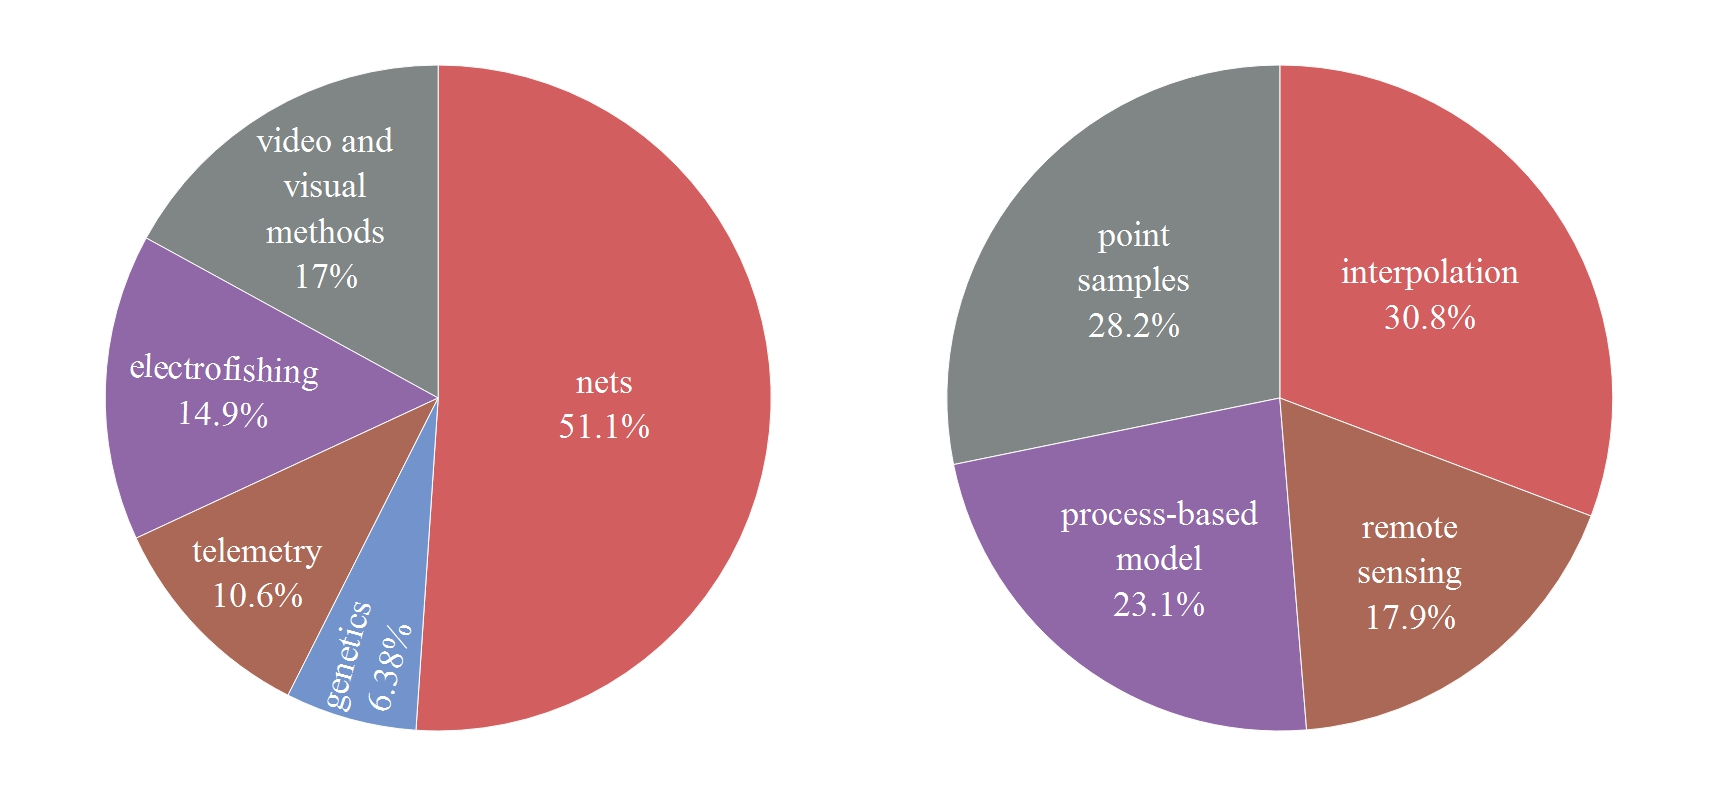
\includegraphics[scale=0.35]{Figure3}
  \caption{Percentage use of different types of biotic and abiotic data acquisition and processing techniques in fish SDM studies which integrated movement. A subset of publications was collected from the Web of Science Core Collection database on the 24\textsuperscript{th} of January 2018 using the following advanced search in title, abstract and keywords: ("species distribution model*" OR "habitat suitability model*" OR "habitat suitability index mapping*" OR "niche model*" OR "species model*" OR "habitat selection model*" OR "resource selection model*" OR "resource model*" OR "gradient analysis*" OR "climate envelope model*" ) AND "fish*" AND ("dispersal*" OR "movement*"). This resulted in a total of 88 publications. From this 88 publications, 54 studies actually involved fish SDM which integrated movement in some way. From this 54 publications only 39 provided a clear description of the used abiotic data acquisition and processing methods while 47 studies provided a clear description of the used biotic data acquisition methods. For the color version of this figure, we refer the reader to the online version of this paper.}
  \label{fig:Figure3}
\end{figure}

\newpage
\begin{landscape}
\begin{table}[ht!]
\begin{center}
\scriptsize
\caption{SWOT analysis of abiotic data acquisition and processing tools for SDM development in aquatic environments. \label{tab:swot}}
\begin{tabular}{|l|l|l|l|l|l|}
\hline
\multicolumn{1}{|c|}{} & \multicolumn{3}{c|}{Independent local point measurements} & \multicolumn{1}{c|}{Remote sensing} & \multicolumn{1}{c|}{Dependent point}\\ 
\hhline{~---~}
\multicolumn{1}{|c|}{} & \multicolumn{1}{c|}{Point-based format} & \multicolumn{2}{c|}{Area-based format} & \multicolumn{1}{c|}{} & \multicolumn{1}{c|}{measurements:}\\
\hhline{~~--~}
\multicolumn{1}{|c|}{} & \multicolumn{1}{c|}{} & \multicolumn{1}{c|}{Geostatistical interpolation} & \multicolumn{1}{c|}{Process-based model} & \multicolumn{1}{c|}{} & \multicolumn{1}{c|}{Animal-borne sensors}\\ 
\hline
\rotatebox{90}{\llap{Strengths~~~~~~~~~}} & \parbox[t]{0.25\textwidth}{%
\begin{itemize}[leftmargin=1em,itemsep=1pt,parsep=0pt]\raggedright%
\item Low degree of processing (uncertainty is only dependent on measurement uncertainty)
\end{itemize}} & \parbox[t]{0.25\textwidth}{%
\begin{itemize}[leftmargin=1em,itemsep=1pt,parsep=0pt]\raggedright%
\item Data driven
\item Spatial correlation
\item Area-based
\item Estimation of uncertainty
\item Inclusion of auxiliary variables 
\end{itemize}} & \parbox[t]{0.25\textwidth}{%
\begin{itemize}[leftmargin=1em,itemsep=1pt,parsep=0pt]\raggedright%
\item Knowledge based
\item Extrapolation
\item Area-based
\end{itemize}} & \parbox[t]{0.25\textwidth}{%
\begin{itemize}[leftmargin=1em,itemsep=1pt,parsep=0pt]\raggedright%
\item Mainly data driven
\item Spatial correlation
\item Area-based
\item Multi-scale
\item Uncertainty is spatially explicit without geographical biases
\end{itemize}} & \parbox[t]{0.25\textwidth}{%
\begin{itemize}[leftmargin=1em,itemsep=1pt,parsep=0pt]\raggedright%
\item Location of measurements depend on location of fish
\item Coinciding scale of abiotic and biotic data
\end{itemize}}\\    \hline
\rotatebox{90}{\llap{Weaknesses~~~~}} & \parbox[t]{0.25\textwidth}{%
\begin{itemize}[leftmargin=1em,itemsep=1pt,parsep=0pt]\raggedright%
\item Point-based (data format is not able to represent geographical space and does not coincide with the biological data format)
\end{itemize}} & \parbox[t]{0.25\textwidth}{%
\begin{itemize}[leftmargin=1em,itemsep=1pt,parsep=0pt]\raggedright%
\item Not well suited for extrapolation
\item No knowledge included
\item Requires awareness model uncertainty
\end{itemize}} & \parbox[t]{0.25\textwidth}{%
\begin{itemize}[leftmargin=1em,itemsep=1pt,parsep=0pt]\raggedright%
\item Inability to capture most biogeochemical fluctuations
\item Requires awareness model uncertainty
\end{itemize}} & \parbox[t]{0.25\textwidth}{%
\begin{itemize}[leftmargin=1em,itemsep=1pt,parsep=0pt]\raggedright%
\item trade-off between spatial, temporal and spectral resolution
\item Cloud cover
\end{itemize}} & \parbox[t]{0.25\textwidth}{%
\begin{itemize}[leftmargin=1em,itemsep=1pt,parsep=0pt]\raggedright%
\item External tagging
\item Tag retrieval is often required to acquire stored data
\end{itemize}}\\    \hline
\rotatebox{90}{~~\llap{Opportunities~~~~~~~~}} & \parbox[t]{0.25\textwidth}{%
\begin{itemize}[leftmargin=1em,itemsep=1pt,parsep=0pt]\raggedright%
\item High temporal resolution
\end{itemize}} & \parbox[t]{0.25\textwidth}{%
\begin{itemize}[leftmargin=1em,itemsep=1pt,parsep=0pt]\raggedright%
\item Biogeochemical variables with many interacting processes
\end{itemize}} & \parbox[t]{0.25\textwidth}{%
\begin{itemize}[leftmargin=1em,itemsep=1pt,parsep=0pt]\raggedright%
\item Hydrodynamical variables with relatively easy to describe processes
\item Physical laws are universal
\end{itemize}} & \parbox[t]{0.25\textwidth}{%
\begin{itemize}[leftmargin=1em,itemsep=1pt,parsep=0pt]\raggedright%
\item New ecologically relevant predictors
\item Combination with local point measurements (i.e. reanalysis products)
\item Rapidly improving technology
\end{itemize}} & \parbox[t]{0.25\textwidth}{%
\begin{itemize}[leftmargin=1em,itemsep=1pt,parsep=0pt]\raggedright%
\item Large fish or mammals, not affected by external tagging
\item Rapidly improving technology
\end{itemize}}\\    \hline
\rotatebox{90}{\llap{Threats~~~~~~}} & \parbox[t]{0.25\textwidth}{%
\begin{itemize}[leftmargin=1em,itemsep=1pt,parsep=0pt]\raggedright%
\item Low spatial resolution
\end{itemize}} & \parbox[t]{0.25\textwidth}{%
\begin{itemize}[leftmargin=1em,itemsep=1pt,parsep=0pt]\raggedright%
\item Importance of distribution of measurement network in time and space
\end{itemize}} & \parbox[t]{0.25\textwidth}{%
\begin{itemize}[leftmargin=1em,itemsep=1pt,parsep=0pt]\raggedright%
\item Unaccounted processes
\end{itemize}} & \parbox[t]{0.25\textwidth}{%
\begin{itemize}[leftmargin=1em,itemsep=1pt,parsep=0pt]\raggedright%
\item Relatively low temporal resolution
\end{itemize}} & \parbox[t]{0.25\textwidth}{%
\begin{itemize}[leftmargin=1em,itemsep=1pt,parsep=0pt]\raggedright%
\item Influence of external tagging on social interaction, swimming speed, etc.
\item Bias towards the tagging of bigger individuals
\end{itemize}}\\    \hline
\end{tabular}
\end{center}
\end{table}
\end{landscape}


%% The Appendices part is started with the command \appendix;
%% appendix sections are then done as normal sections
%% \appendix

%% \section{}
%% \label{}

%% References
%%
%% Following citation commands can be used in the body text:
%% Usage of \citep is as follows:
%%   \citep{key}          ==>>  [#]
%%   \citep[chap. 2]{key} ==>>  [#, chap. 2]
%%   \citept{key}         ==>>  Author [#]

%% References with bibTeX database:

%\biboptions{square,sort,comma,numbers}
\bibliographystyle{elsarticle-harv-noURL}
\newpage
\section*{References}
\bibliography{My_Collection.bib}

%% Authors are advised to submit their bibtex database files. They are
%% requested to list a bibtex style file in the manuscript if they do
%% not want to use model1-num-names.bst.

%% References without bibTeX database:

% \begin{thebibliography}{00}

%% \bibitem must have the following form:
%%   \bibitem{key}...
%%

% \bibitem{}

% \end{thebibliography}


\end{document}

%%
%% End of file `elsarticle-template-1-num.tex'.